\documentclass[onecolumn, draftclsnofoot,10pt, compsoc]{IEEEtran}
\usepackage{graphicx}
\usepackage{url}
\usepackage{setspace}
\usepackage{geometry}
\usepackage{tabularx}
\geometry{textheight=9.5in, textwidth=7in}

\def \CapstoneTeamName{		    Comedy Robot Team}
\def \CapstoneTeamNumber{		43}
\def \GroupMemberOne{			Timothy Bui}
\def \GroupMemberTwo{			Yuhang (Tony) Chen}
\def \GroupMemberThree{			Brian Ozarowicz}
\def \GroupMemberFour{			Trevor Webster}
\def \CapstoneProjectName{		Building More Self-Aware\linebreak Everyday Robots}
\def \CapstoneSponsorCompany{	SHARE Lab}
\def \CapstoneSponsorPerson{	Dr. Naomi Fitter}

% Uncomment the appropriate line below so that the document type works
\def \DocType{	%Problem Statement
				%Requirements Document
				%Technology Review
				%Design Document
				Progress Report
				}
			
\newcommand{\NameSigPair}[1]{\par
\makebox[2.75in][r]{#1} \hfil 	\makebox[3.25in]{\makebox[2.25in]{\hrulefill} \hfill		\makebox[.75in]{\hrulefill}}
\par\vspace{-12pt} \textit{\tiny\noindent
\makebox[2.75in]{} \hfil		\makebox[3.25in]{\makebox[2.25in][r]{Signature} \hfill	\makebox[.75in][r]{Date}}}}
% If the document is not to be signed, uncomment the RENEWcommand below
\renewcommand{\NameSigPair}[1]{#1}

%%%%%%%%%%%%%%%%%%%%%%%%%%%%%%%%%%%%%%%
\begin{document}
\begin{titlepage}
    \pagenumbering{gobble}
    \begin{singlespace}
    	
\includegraphics[height=4cm]{coe_v_spot1}
        \hfill 
        % If you have a logo, use this includegraphics command to put it on the coversheet.
        %\includegraphics[height=4cm]{CompanyLogo}   
        \par\vspace{.2in}
        \centering
        \scshape{
            \huge CS Capstone \DocType \par
            %{\large\today}\par
            {\large Winter 2020}\par
            \vspace{.5in}
            \textbf{\Huge\CapstoneProjectName}\par
            \vfill
            {\large Prepared for}\par
            %\Huge \CapstoneSponsorCompany\par
            %\vspace{5pt}
            {\Large\NameSigPair{\CapstoneSponsorPerson}\par}
            {\large Prepared by }\par
            Group\CapstoneTeamNumber\par
            % comment out the line below this one if you do not wish to name your team
            \CapstoneTeamName\par 
            \vspace{5pt}
            {\Large
                \NameSigPair{\GroupMemberOne}\par
                \NameSigPair{\GroupMemberTwo}\par
                \NameSigPair{\GroupMemberThree}\par
                \NameSigPair{\GroupMemberFour}\par
            }
            \vspace{20pt}
        }
        \begin{abstract}
        	\noindent This document provides a summary of the progress made during Winter term on the 'Building More Self-Aware Everyday Robots' Capstone project. It describes the code development that has been done in relation to the established project goals and gives the plan for upcoming implementation onto hardware and project stretch goals.
        \end{abstract}
    \end{singlespace}
\end{titlepage}
\newpage
\pagenumbering{arabic}
\tableofcontents
% uncomment this (if applicable). Consider adding a page break.
%\listoffigures
%\listoftables
\clearpage

\section{Purpose and Goals}
The purpose of our project is to study how human-robot interactions can be improved by observing the ability of a robotic stand-up comedian to read and respond to cues from its audience. Our goals are to use machine learning on a dataset of recordings from previous comedy performances to train models for detecting laughter and using that response to decide whether a joke was a hit or a bomb.\par
\vspace{.3cm}
\noindent This analysis can be used by the robot to make real-time adjustments to its performance based on the perceived audience preferences in order to improve the success of their interpersonal communications. The work also has potential applications outside the field of comedy in improving the experience of interactions with AI assistants and other autonomous systems.

\section{Terminology}
\vspace{.5cm}
\fbox{\begin{minipage}{\linewidth}
\vspace{.2cm}
{\bf Performance:} The audio data recorded by the robot during its stand-up comedy routine. Each performance contains multiple jokes and every joke has a corresponding audience response. The audio for each joke is split into the following two files:
\begin{itemize}
\item {\bf Joke Audio:} The audio in the period of time in a performance where the robot is telling a joke
\item {\bf Post-Joke Audio:} The audience's reaction to the joke; consisting of the audio from the time after the joke finished until the time when the next joke starts being told
\end{itemize}
\hrule \vspace{.3cm}
{\bf Audience Response:} The audience's response to a joke told during a performance. The response can be categorized in one of the three following ways:
\begin{itemize}
\item {\bf Positive Response:} Laughter in chorus from the crowd
\item {\bf Neutral Response:} Laughter from an individual audience member or quiet and scattered laughter
\item {\bf Negative Response:} Silence or relative silence from the crowd
\end{itemize}
\hrule \vspace{.3cm}
{\bf 3-Class:} The division of the jokes into negative responses (-1), neutral responses (0), and positive responses (1)
\vspace{.2cm} \hrule \vspace{.3cm}
{\bf 2-Class:} The division of the jokes between negative responses (0) and neutral or positive responses (1)
\vspace{.2cm} \hrule \vspace{.3cm}
{\bf Feature:} Specific information extracted from audio that is used to train the classifier
\vspace{.2cm} \hrule \vspace{.3cm}
{\bf Praat:} Software used to extract features from the audio
\vspace{.2cm} \hrule \vspace{.3cm}
{\bf Human Rating:} The result from a single human rating each individual joke based on how they would perceive the audience's response if they were giving a stand-up comedy performance
\vspace{.2cm} \hrule \vspace{.3cm}
{\bf Ground Truth Rating:} The rating found by taking the median of the individual human ratings for each joke
\end{minipage}}
\clearpage
\fbox{\begin{minipage}{\linewidth}
\vspace{.2cm}
{\bf Post-Joke Classifier:} The classifier which tries to determine the audience response in the post-joke audio file. It uses the following features:
\begin{itemize}
\item {\bf Pitch:} The mean frequency of the audio file, measured in Hertz
\item {\bf PitchSd:} The standard deviation of the frequency of the audio file, measured in Hertz
\item {\bf Intensity:} The mean amplitude of the audio file, measured in decibels
\item {\bf IntensitySd:} The standard deviation of the amplitude of the audio file, measured in decibels
\item {\bf MaxSound:} The maximum amplitude of the audio file, measured in Sinc70
\item {\bf MinSound:} The minimum amplitude of the audio file, measured in Sinc70
\end{itemize}
\hrule \vspace{.3cm}
{\bf Mid-Joke Classifier:} The classifier which tries to determine the audience response in the joke audio file. It uses the following features:
\begin{itemize}
\item {\bf Min\_Pitch:} The minimum pitch of the the audio file, measured in Hertz
\item {\bf Max\_Pitch:} The maximum pitch of the the audio file, measured in Hertz
\item {\bf Mean\_Pitch:} The average pitch of the the audio file, measured in Hertz
\item {\bf SD\_Pitch:} The standard deviation of the pitch of the the audio file, measured in Hertz
\item {\bf Min\_Intensity:} The minimum amplitude of the audio file, measured in decibels
\item {\bf Max\_Intensity:} The maximum amplitude of the audio file, measured in decibels
\item {\bf Mean\_Intensity:} The average amplitude of the audio file, measured in decibels
\item {\bf SD\_Intensity:} The standard deviation of the amplitude of the audio file, measured in decibels
\end{itemize}
\end{minipage}}
\vspace{.1cm}

\section{Current Status}
We had three team members assign human ratings to the jokes in our dataset and averaged those ratings to produce our initial ground truth ratings for use training our classifiers. The results were later found to be invalid for use in the machine learning phase of the project, for reasons detailed in the Problems section of this report, however they were still able to be used to calculate the human rater accuracy level which could be used as a benchmark for our classifier results. A single team member then rerated all the jokes to produce a valid ground truth file for use with the classifiers.\par
\vspace{.3cm}
\noindent We have implemented separate classifiers for the mid-joke and post-joke analysis which determine whether laughter occurred or not while the joke was being told and after the joke concluded respectively. The classifiers can use several different learning models; the accuracy rates achieved by each model are shown in the Results section of this report. The post-joke classifier can operate as both 3-Class - categorizing the audience response as positive, negative, or neutral - or 2-Class - categorizing as either laughter present or not present. The mid-joke classifier is only 2-Class - simply deciding whether laughter, of any type, was detected during the telling of the joke.

\section{Work Remaining}
In regard to the official project deliverables established in our documentation last term what remains is to combine the mid-joke and post-joke analysis pieces to produce one overall joke rating from our classifier, then implement the classifier onto the robot hardware and test its use in real-time operation. After this is achieved we have some potential stretch goals to begin work on which are beyond the scope of the course grading criteria, but will be extra production to come out of this project to assist our client in future development.\par
\vspace{.3cm}
\noindent One goal is to migrate the robot's programming from the current use of a program called Choregraphe to using the Python SDK. This will allow for better adaptability in future programming of the robot's performance as Choregraphe has become difficult to use as the routine becomes gradually more complex.\par
\vspace{.3cm}
\noindent Other potential stretch goals include conducting human trials of live performances using the new classifier to observe its decision making ability in real-world operation compared to over the previously recorded dataset, as well as preparing the presentation of our results to be the foundation of a new research paper.

\section{Problems and Solutions}
The original classifier program provided by the client from a previous team's work assumed the jokes were being read in from the ratings csv in the order they had been told during the performance. Our ratings were generated using an annotator program that the previous team did not use, so our jokes were actually randomly ordered. This resulted in the classifier incorrectly matching the featurue data from the Praat files to the joke names, producing invalid results. Once this issue was identified we added new functionality to the classifier to ensure the randomly ordered jokes were assigned their correct Praat data before the machine learning was performed.\par
\vspace{.3cm}
\noindent A bug was found in the annotator program that caused it to skip the audio files for jokes that were follow-up tags, causing our ratings to be incomplete. We notified the client and the issue was quickly fixed. We then reran the annotator to produce ratings for the audio that had been skipped before to complete the human ratings csv.\par
\vspace{.3cm}
\noindent It was later noticed that the annotator was not correctly matching some joke names to the ratings they should have. Investigation found that this was happening because it was not actually playing all of the audio files from a performance, but was replaying half of the files twice and giving their ratings to joke names that never had their corresponding audio played. The result was that the ground truths we had been using were invalid as there was no way to determine which ratings were matched to their correct jokes. After discussion with the client it was determined that the cause of this bug would be too difficult to track down to be worth the time it would take away from proceeding with the rest of the project. The solution arrived at was for one human to redo all the joke ratings by hand to produce a ground truths csv that we knew was complete and correct.

\section{Results}
This section describes the preliminary results from our work on the post-joke and mid-joke classification and includes some data visualization graphs produced from both parts of the project.

\subsection{Post-Joke Analysis}
For a 3-Class division of the data we have two datasets where three human raters have listened to the post-joke audio and rated the audience response then these three human ratings were combined to form a ground truth rating. In the first dataset the individual human ratings matched the ground truths with accuracy rates of 82\%, 84\%, and 87\%. In the second dataset the human ratings matched the ground truths with accuracy rates of 69\%, 70\%, and 89\%. Based on these results we determined that our original goal of an accuracy rating of 85\% for the post-joke classifier compared to the ground truth ratings would be reasonable, since this is about equivalent to what we would expect from a human classifying the data.\par
\vspace{.3cm}
\noindent We used two validation techniques with our classifiers. The first approach is to leave the data from one performance out for validation then train the classifier using the data from the remaining performances. We repeated this for each performance and took the mean accuracy across the classifiers as our final accuracy value. The second approach is holding out 20\% of the data, randomly selected from across the entire dataset, then training the classifiers on the remaining 80\% of the data. We repeated this process 100 times and took the average accuracy across all the trials as our final value.\par
\vspace{.3cm}
\noindent At our current standing in the project we have achieved our goal with an accuracy rating of around 85\% using leave one performance out validation and around 88\% using hold out 20\% validation with our best classifier and around 83-86\% accuracy with all classifiers. The individual accuracy results for each classifier are shown in the images provided later in this section. These results seem to indicate that the classifier is able to detect laughter from an audience in a stand-up comedy environment with about the same level of accuracy as a human.\par
\vspace{.3cm}
\noindent There are some limitations to the current results and scope of the project. For example, we were working with a limited sample size of the number of human raters, the number of performances, and the number of performance environments. We have also been unable to test the classifier in a real world environment. As we implement the classifier onto the robot hardware and conduct live performance tests we can determine if there is a significant difference in the real-time operation compared to operating over the dataset of pre-recorded audio.

\subsection{Mid-Joke Analysis}
For the mid-joke 2-Class division of data we had one dataset where one human rated all of the audio clips. We chose to do it this way because at the time we were unsure if our method would prove to be successful and wanted to keep this task as cheap as possible in the time investment required. When annotating the audio we simply looked for if there was laughter heard or not, regardless of its qualities, hence the 2-Class division being sufficient.\par
\vspace{.3cm}
\noindent We used leave-one-out validation to verify the accuracy of our classifiers. Similarly to the post-joke validation, we would leave the data for one full performance out and train the classifier using the data from the other performances. This was then repeated for all the performances in the dataset and the mean accuracy across all performances was used to determine our final accuracy.\par
\vspace{.3cm}
\noindent Currently we have around 73\% accuracy with the Gaussian Radial Basis Function (RBF) kernel in our support vector machine (SVM) model. While this is not completely accurate by human standards, it should give us a good enough reading on whether the audience laughed mid-joke or not. When combined with the post-joke analysis the laughter detection should be more than sufficient to make an overall decision for the joke.

\clearpage
\subsection{Data Visualization}

\begin{figure}[!h]
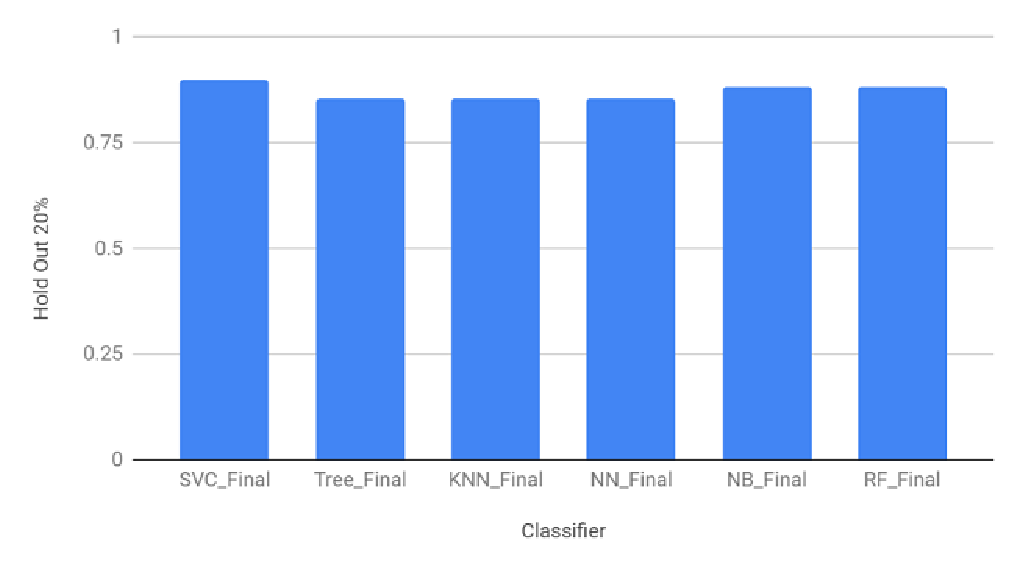
\includegraphics[width=\linewidth]{assets/results1.eps}
\caption{Classifier Results}
\end{figure}

\begin{figure}[!h]
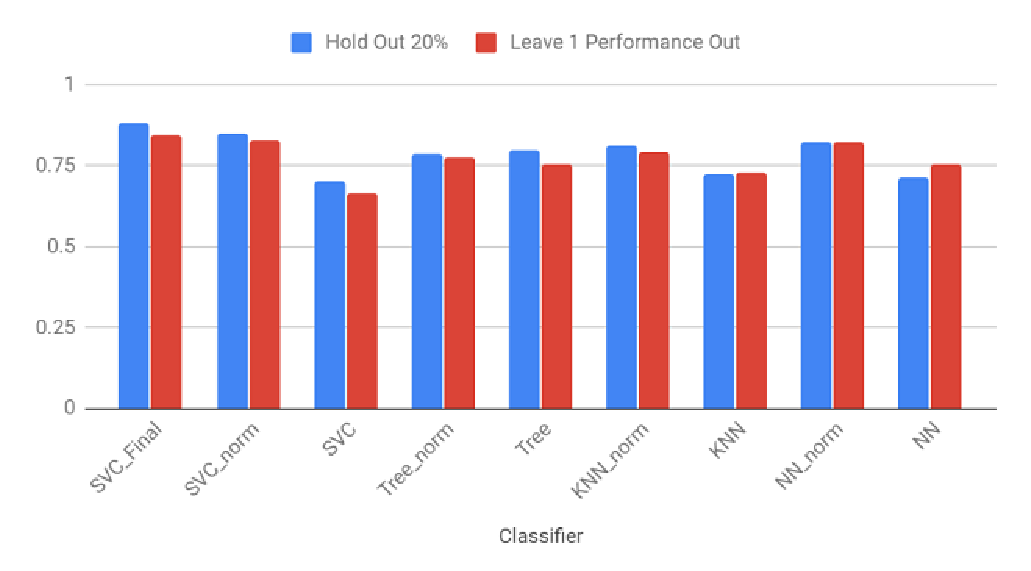
\includegraphics[width=\linewidth]{assets/results2.eps}
\caption{Classifier Accuracy}
\end{figure}

\begin{figure}[!h]
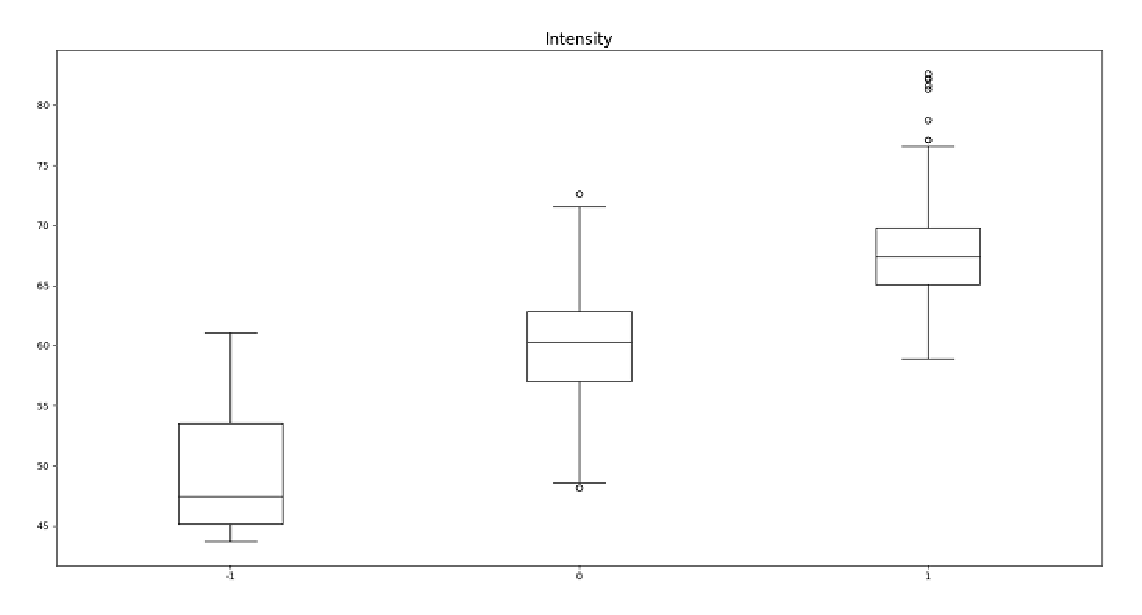
\includegraphics[width=\linewidth]{assets/fig1.eps}
\caption{Distribution of Intensity based on Ground Truth Ratings for Post-Joke Audio}
\end{figure}

\begin{figure}[!h]
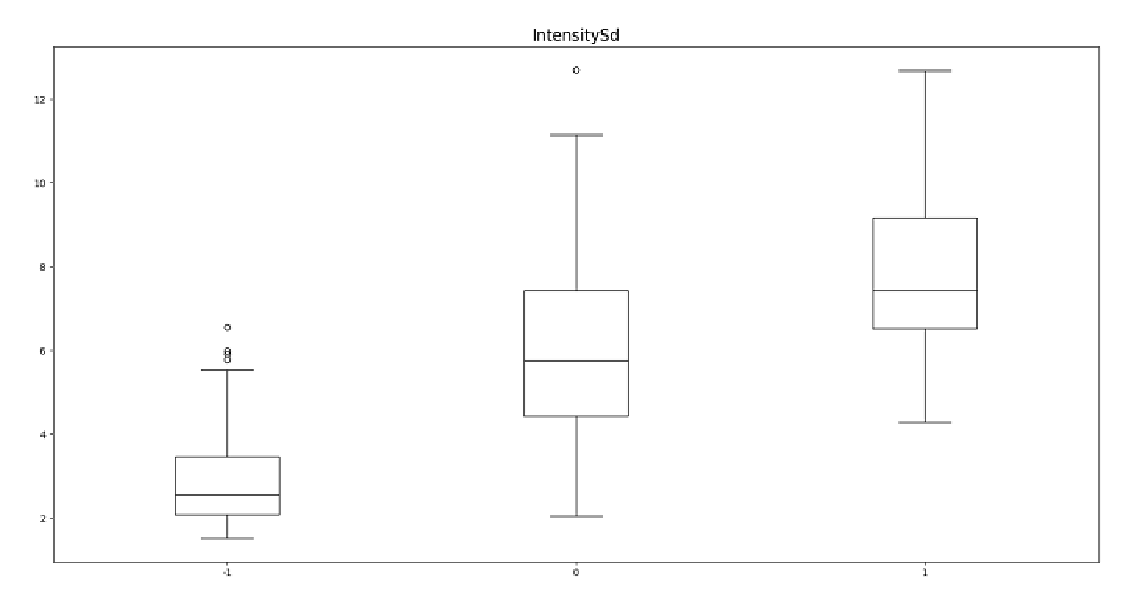
\includegraphics[width=\linewidth]{assets/fig2.eps}
\caption{Distribution of Intensity Standard Deviation based on Ground Truth Ratings for Post-Joke Audio}
\end{figure}

\begin{figure}[!h]
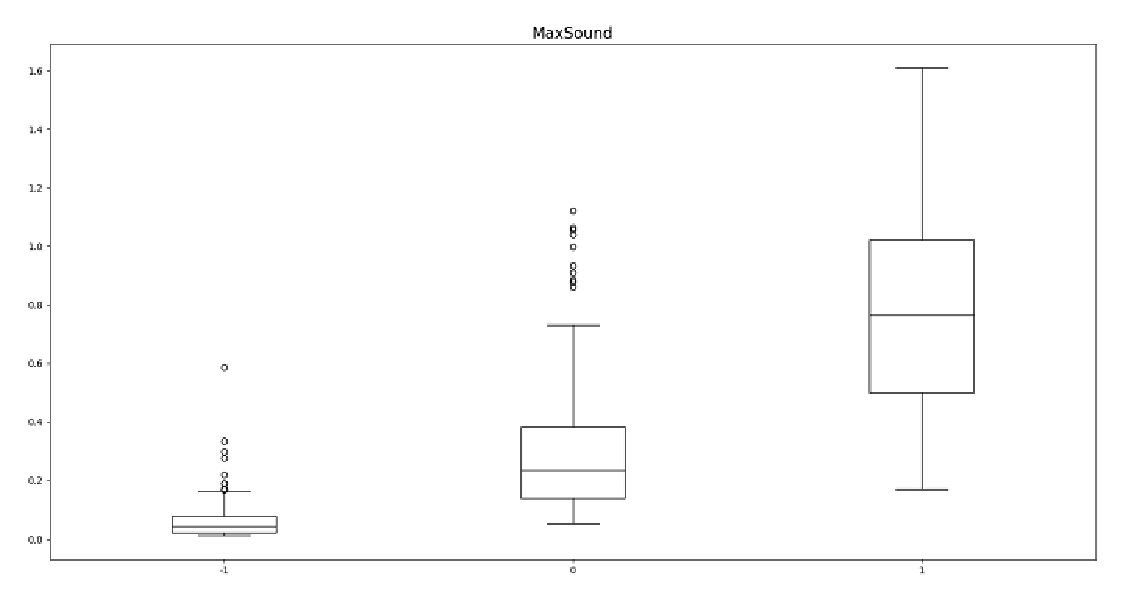
\includegraphics[width=\linewidth]{assets/fig3.eps}
\caption{Distribution of Max Sound based on Ground Truth Ratings for Post-Joke Audio}
\end{figure}

\begin{figure}[!h]
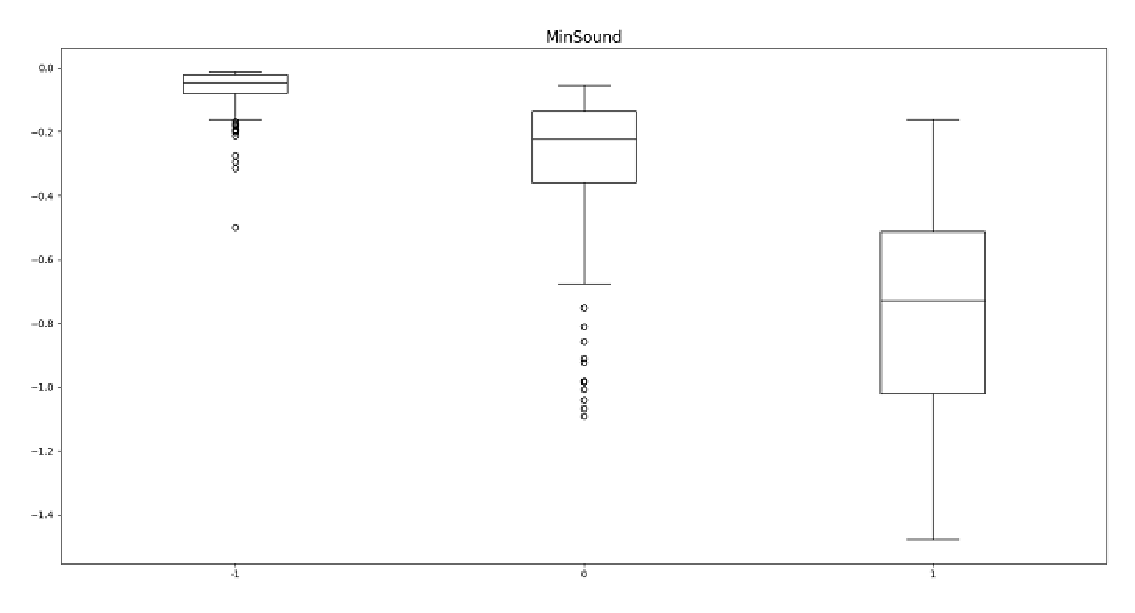
\includegraphics[width=\linewidth]{assets/fig4.eps}
\caption{Distribution of Min Sound based on Ground Truth Ratings for Post-Joke Audio}
\end{figure}

\begin{figure}[!h]
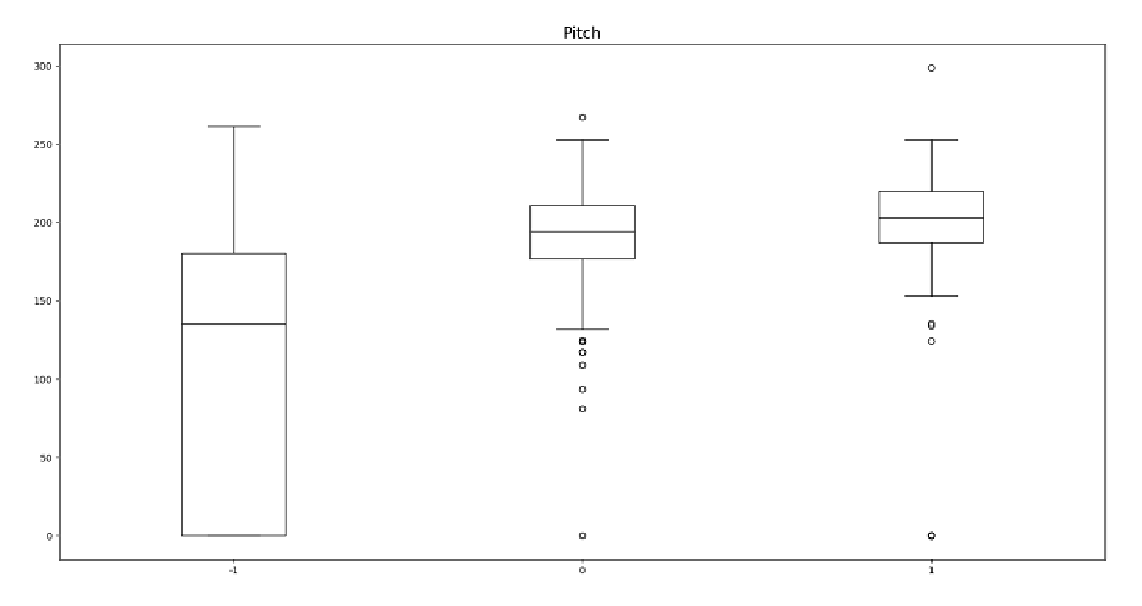
\includegraphics[width=\linewidth]{assets/fig5.eps}
\caption{Distribution of Pitch based on Ground Truth Ratings for Post-Joke Audio}
\end{figure}

\begin{figure}[!h]
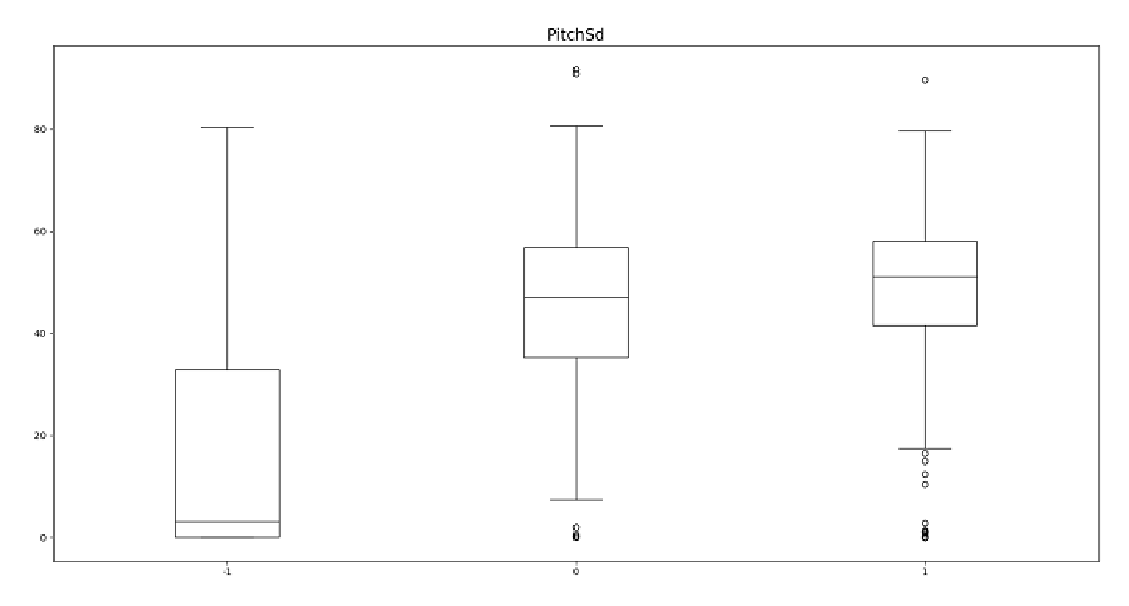
\includegraphics[width=\linewidth]{assets/fig6.eps}
\caption{Distribution of Pitch Standard Deviation based on Ground Truth Ratings for Post-Joke Audio}
\end{figure}

\begin{figure}[!h]
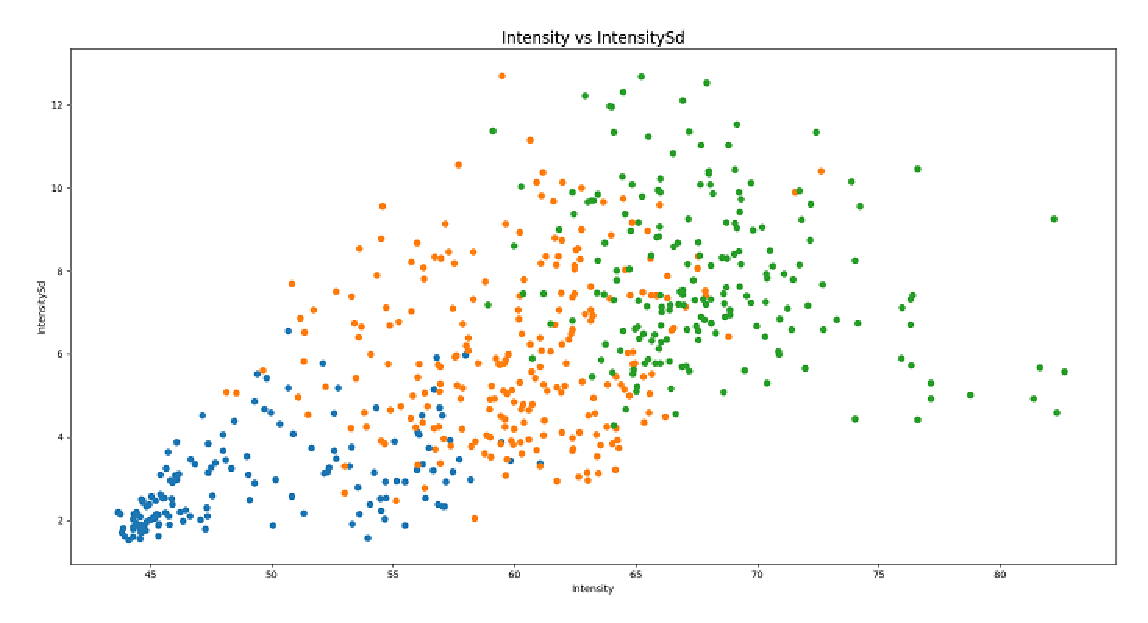
\includegraphics[width=\linewidth]{assets/fig7.eps}
\caption{Ground Truth Ratings Visualized by Intensity vs Intensity Standard Deviation for Post-Joke Audio}
\end{figure}

\begin{figure}[!h]
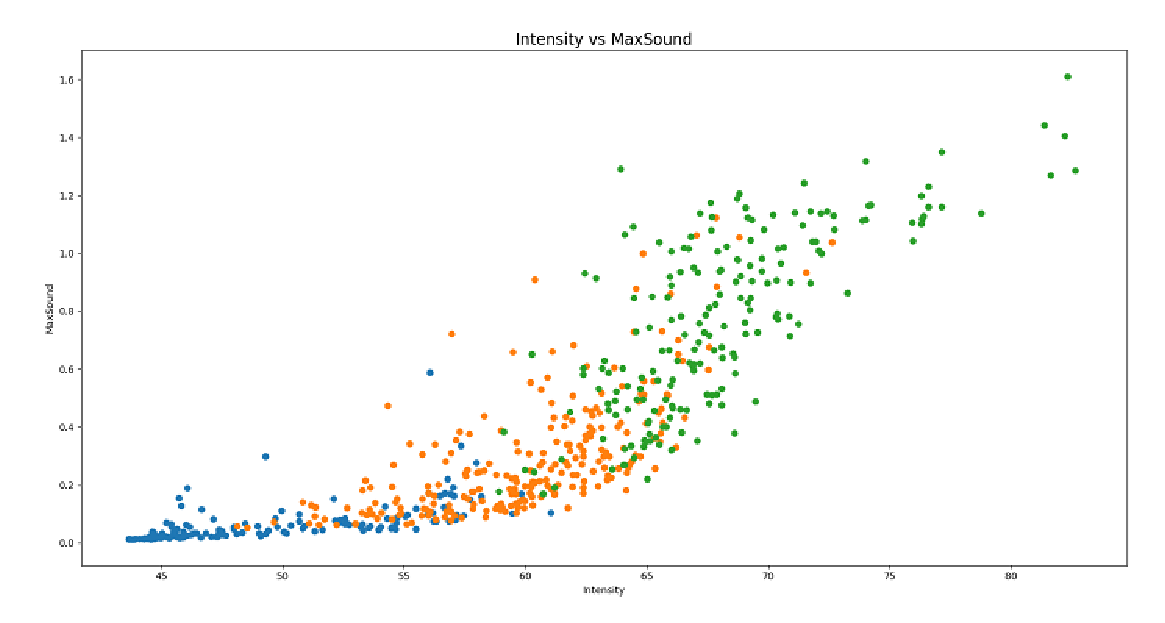
\includegraphics[width=\linewidth]{assets/fig8.eps}
\caption{Ground Truth Ratings Visualized by Intensity vs Max Sound for Post-Joke Audio}
\end{figure}

\begin{figure}[!h]
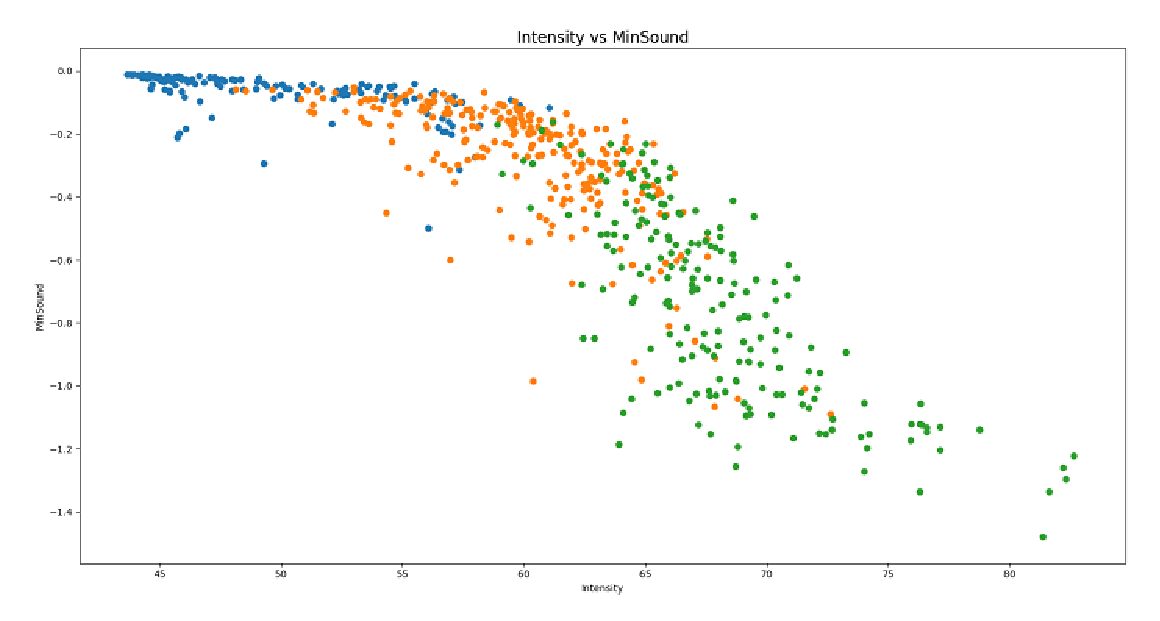
\includegraphics[width=\linewidth]{assets/fig9.eps}
\caption{Ground Truth Ratings Visualized by Intensity vs Min Sound for Post-Joke Audio}
\end{figure}

\begin{figure}[!h]
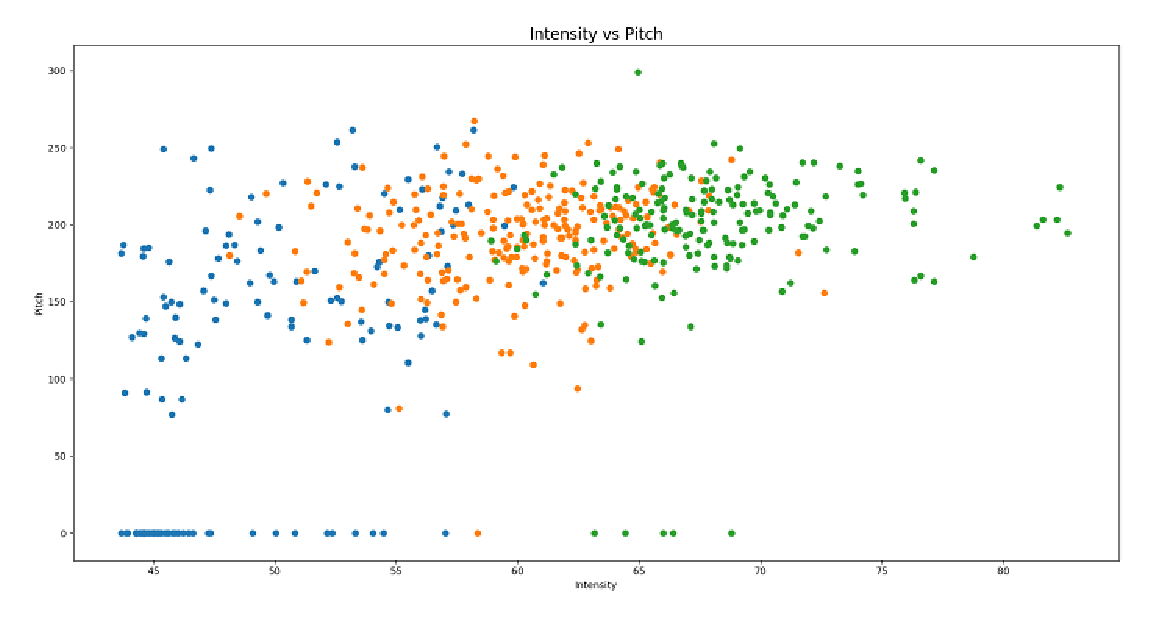
\includegraphics[width=\linewidth]{assets/fig10.eps}
\caption{Ground Truth Ratings Visualized by Intensity vs Pitch for Post-Joke Audio}
\end{figure}

\begin{figure}[!h]
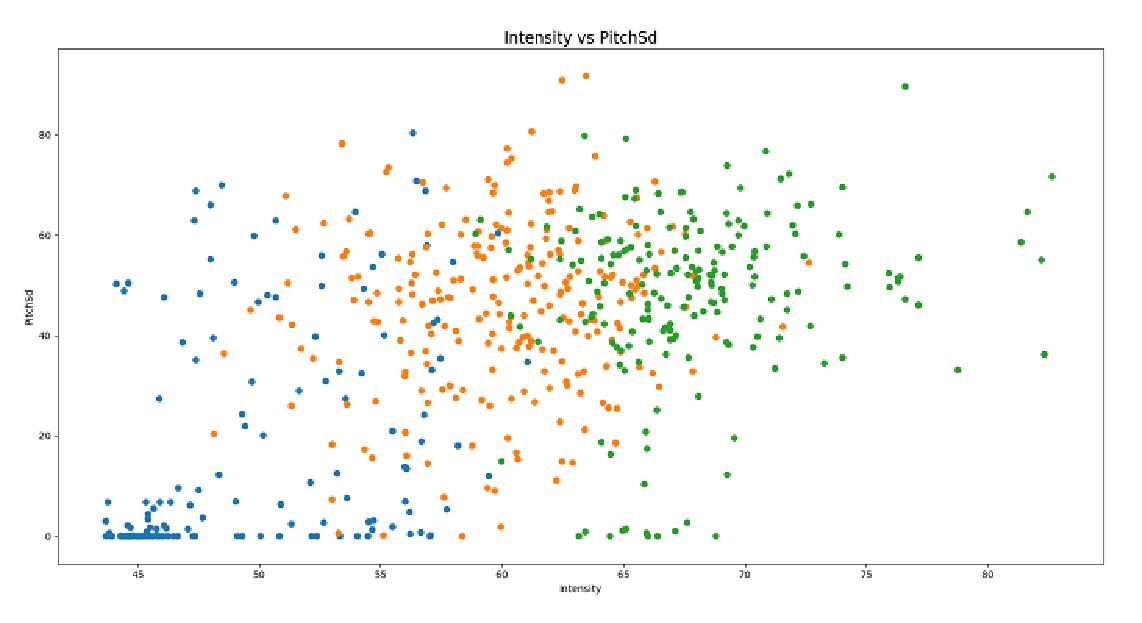
\includegraphics[width=\linewidth]{assets/fig11.eps}
\caption{Ground Truth Ratings Visualized by Intensity vs Pitch Standard Deviation for Post-Joke Audio}
\end{figure}

\begin{figure}[!h]
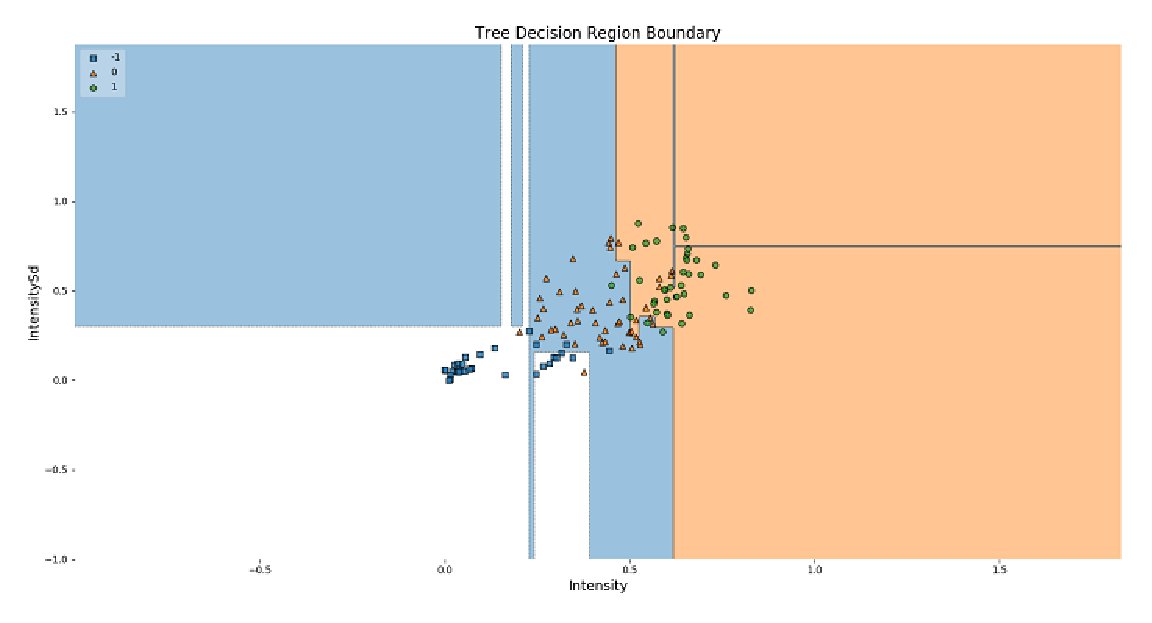
\includegraphics[width=\linewidth]{assets/fig12.eps}
\caption{Decision Boundaries for Decision Tree Classifier Visualized by Intensity vs Intensity Standard Deviation for Post-Joke Classifier}
\end{figure}

\begin{figure}[!h]
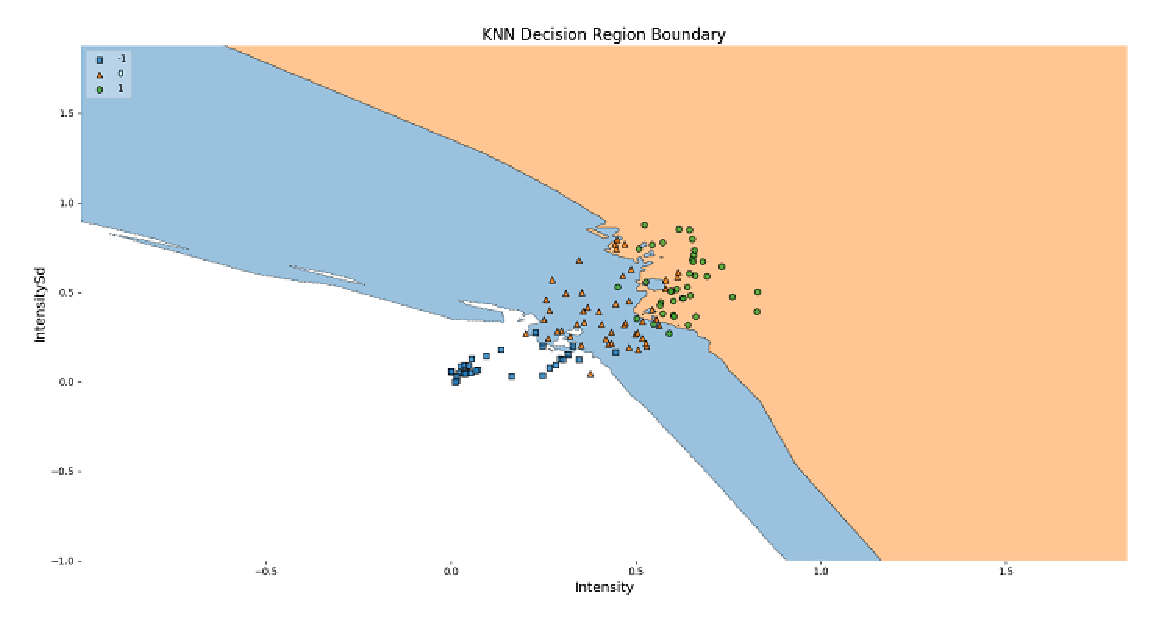
\includegraphics[width=\linewidth]{assets/fig13.eps}
\caption{Decision Boundaries for K Nearest Neighbor Classifier Visualized by Intensity vs Intensity Standard Deviation for Post-Joke Classifier}
\end{figure}

\begin{figure}[!h]
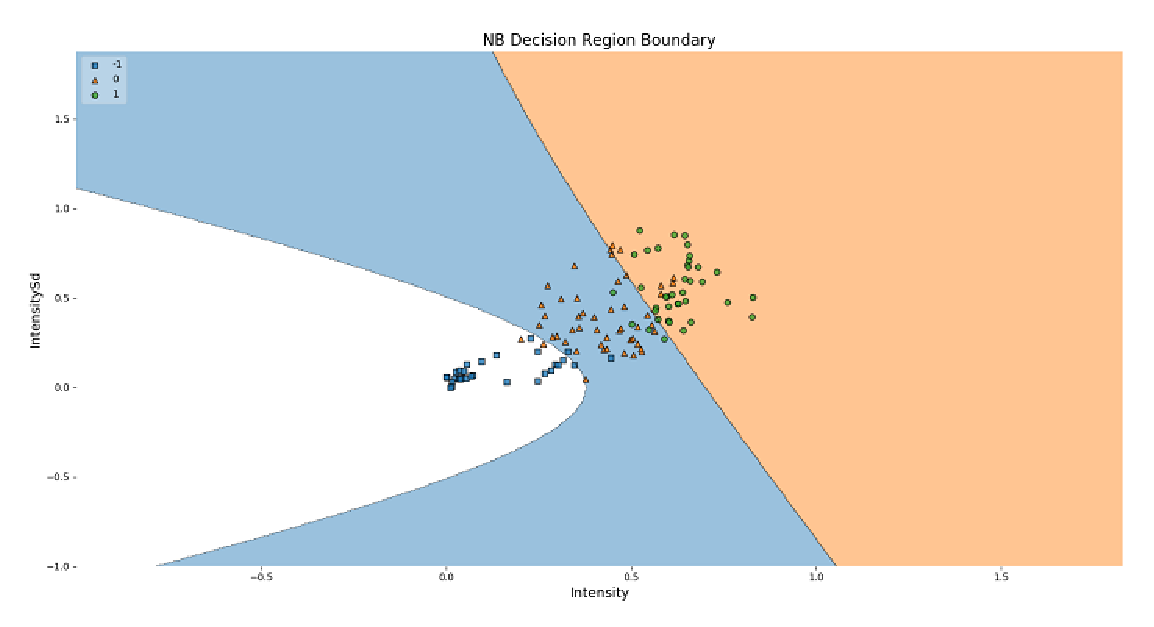
\includegraphics[width=\linewidth]{assets/fig14.eps}
\caption{Decision Boundaries for Naive Bayes Classifier Visualized by Intensity vs Intensity Standard Deviation for Post-Joke Classifier}
\end{figure}

\begin{figure}[!h]
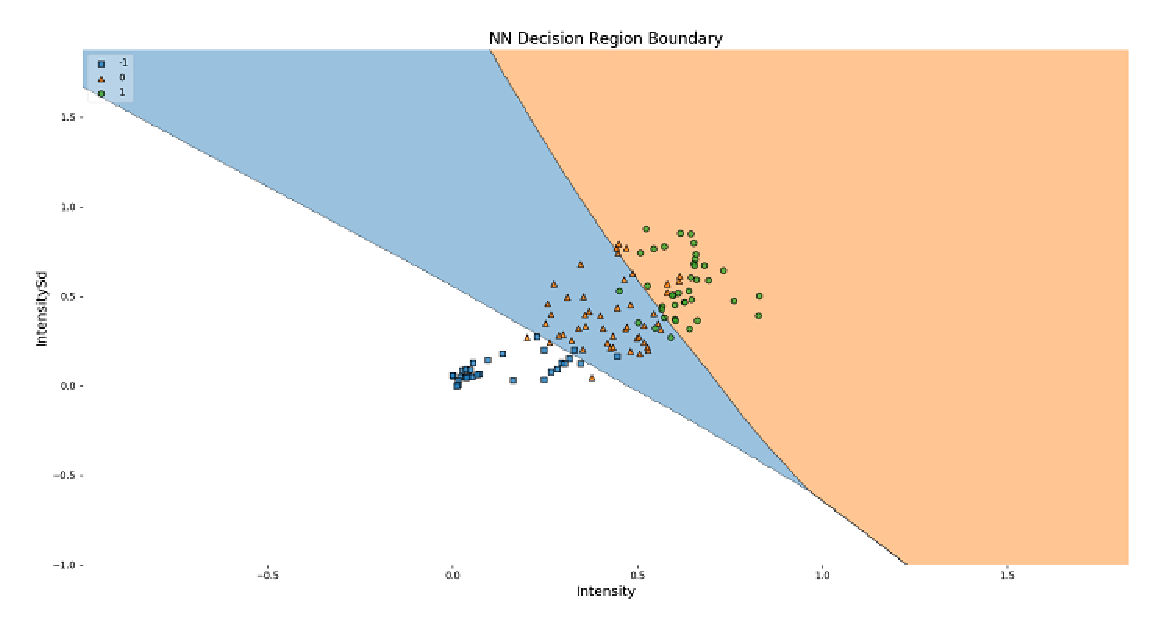
\includegraphics[width=\linewidth]{assets/fig15.eps}
\caption{Decision Boundaries for Neural Network Classifier Visualized by Intensity vs Intensity Standard Deviation for Post-Joke Classifier}
\end{figure}

\begin{figure}[!h]
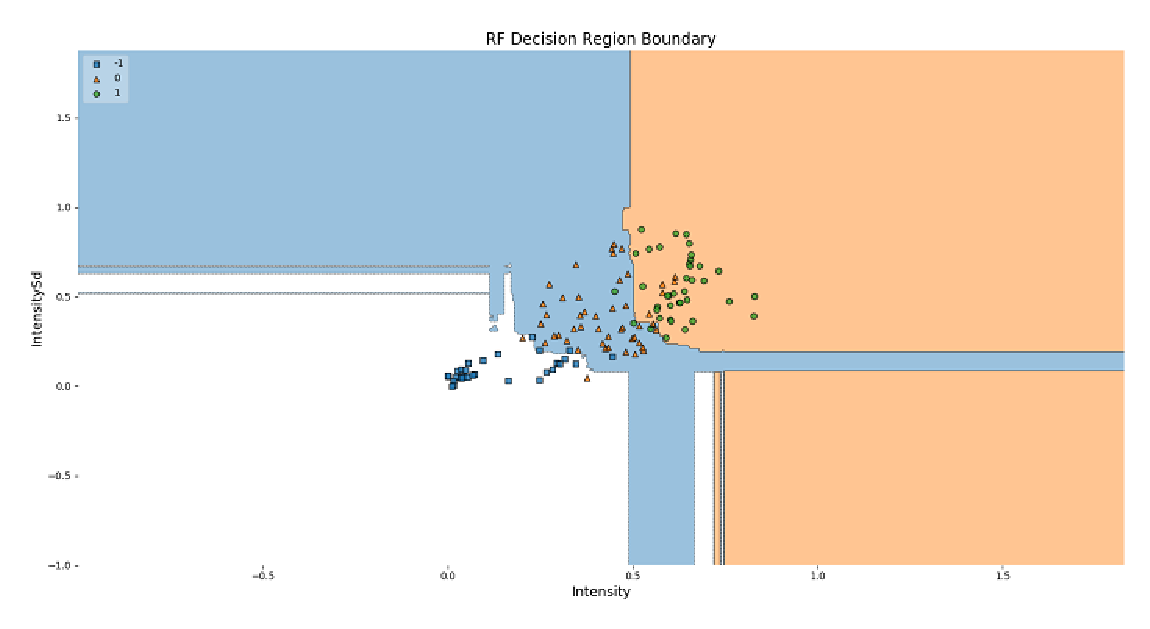
\includegraphics[width=\linewidth]{assets/fig16.eps}
\caption{Decision Boundaries for Random Forest Classifier Visualized by Intensity vs Intensity Standard Deviation for Post-Joke Classifier}
\end{figure}

\begin{figure}[!h]
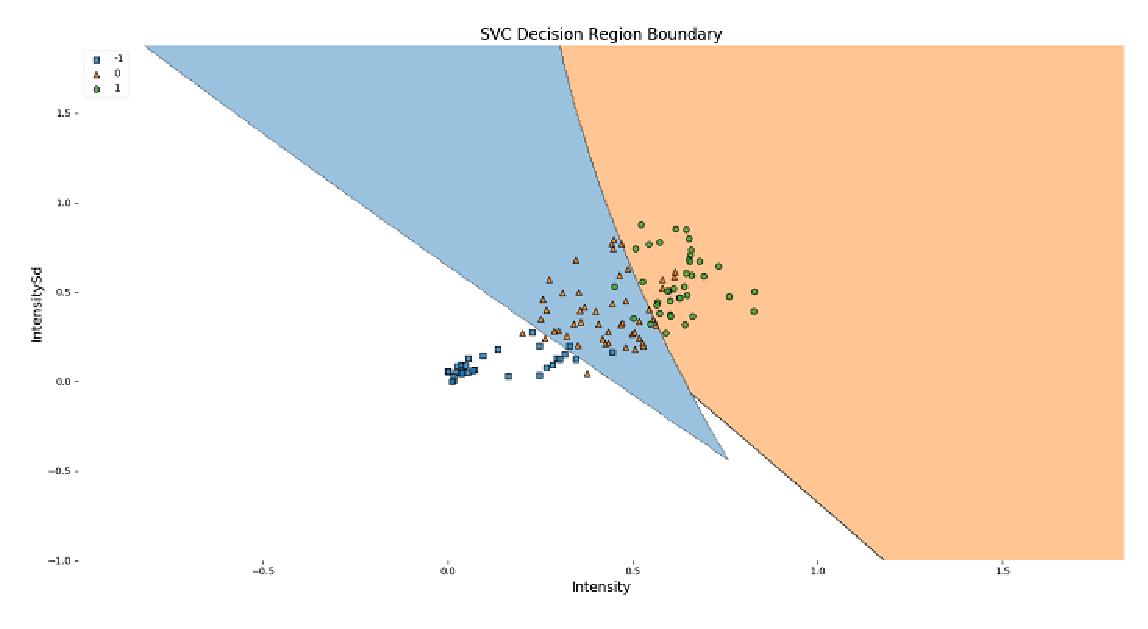
\includegraphics[width=\linewidth]{assets/fig17.eps}
\caption{Decision Boundaries for Support Vector Classifier Visualized by Intensity vs Intensity Standard Deviation for Post-Joke Classifier}
\end{figure}

\begin{figure}[!h]
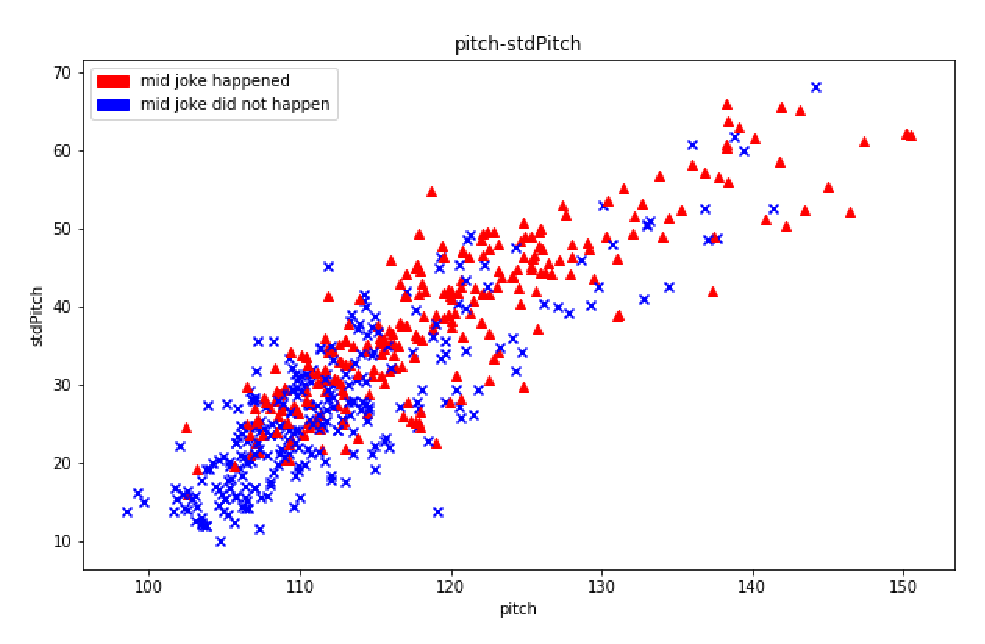
\includegraphics{assets/fig18.eps}
\caption{Positive Correlation of Pitch and Standard Deviation Pitch in Mid-Joke Audio Overall}
\end{figure}

\begin{figure}[!h]
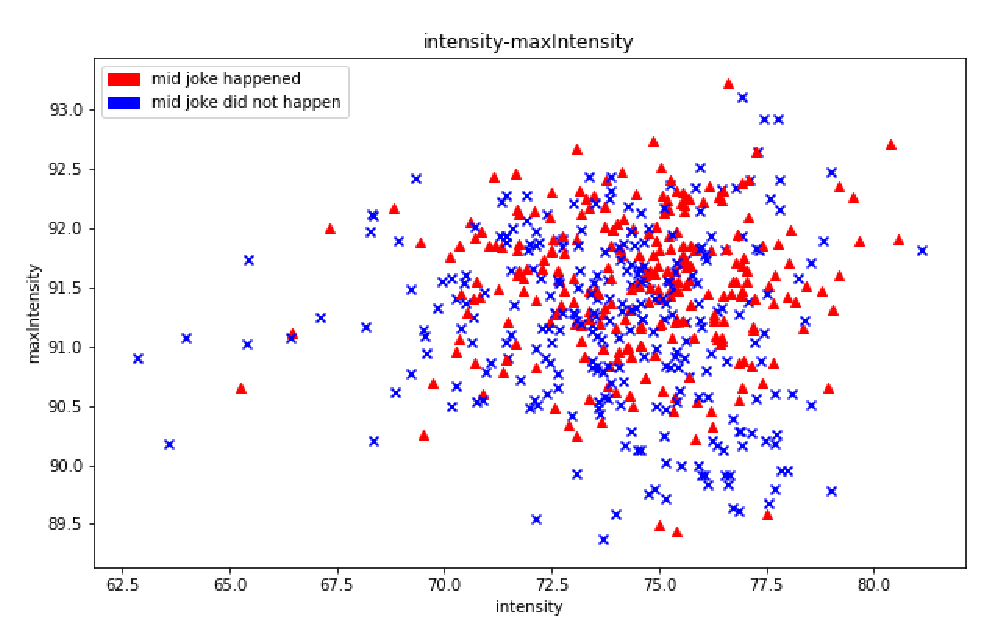
\includegraphics{assets/fig19.eps}
\caption{No Correlation of Intensity and Max Intensity in Mid-Joke Audio Overall}
\end{figure}

\begin{figure}[!h]
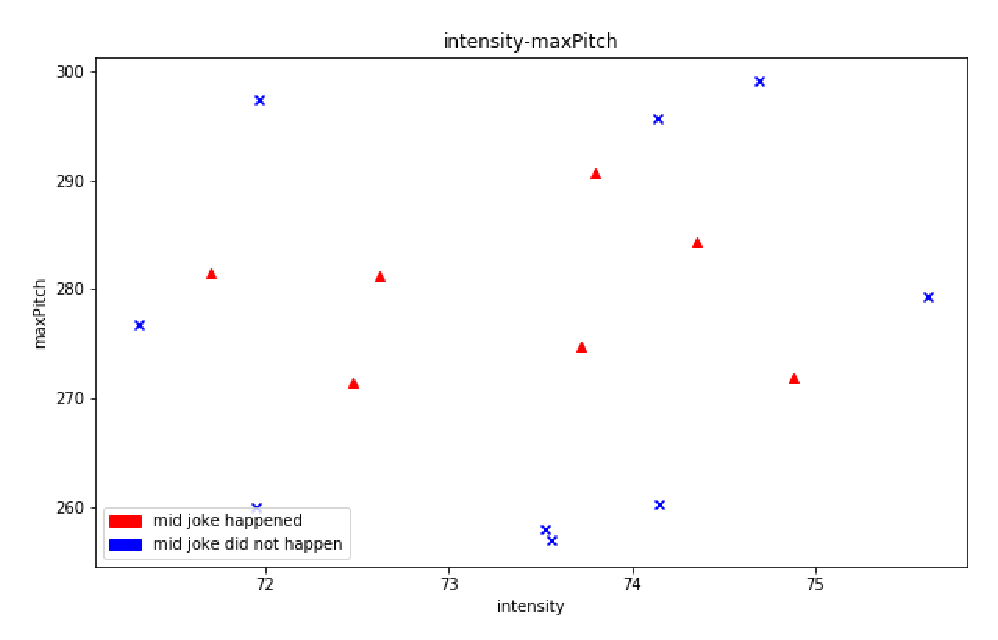
\includegraphics{assets/fig20.eps}
\caption{No Correlation of Intensity and Max Intensity in Mid-Joke Audio Compared Joke-wise}
\end{figure}

\begin{figure}[!h]
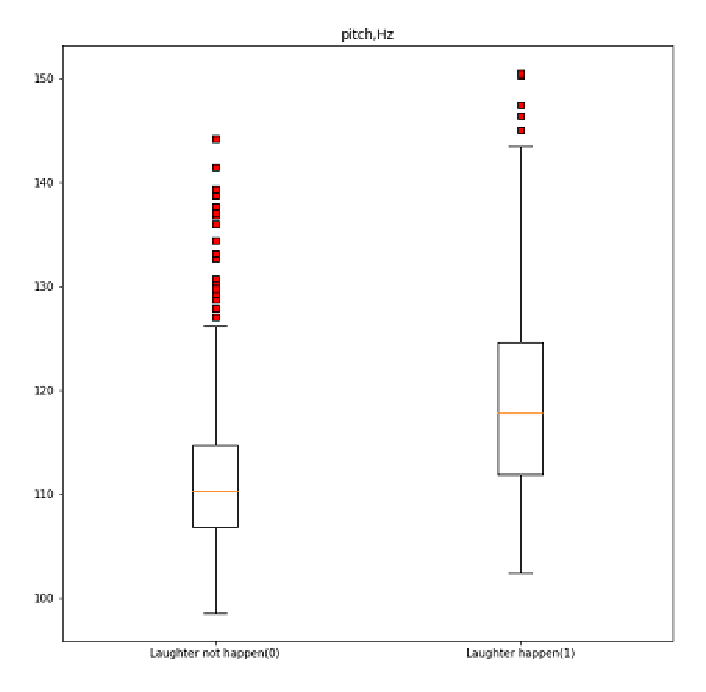
\includegraphics{assets/fig21.eps}
\caption{Distribution of Pitch based on Ground Truth Ratings for Mid-Joke Audio}
\end{figure}

\begin{figure}[!h]
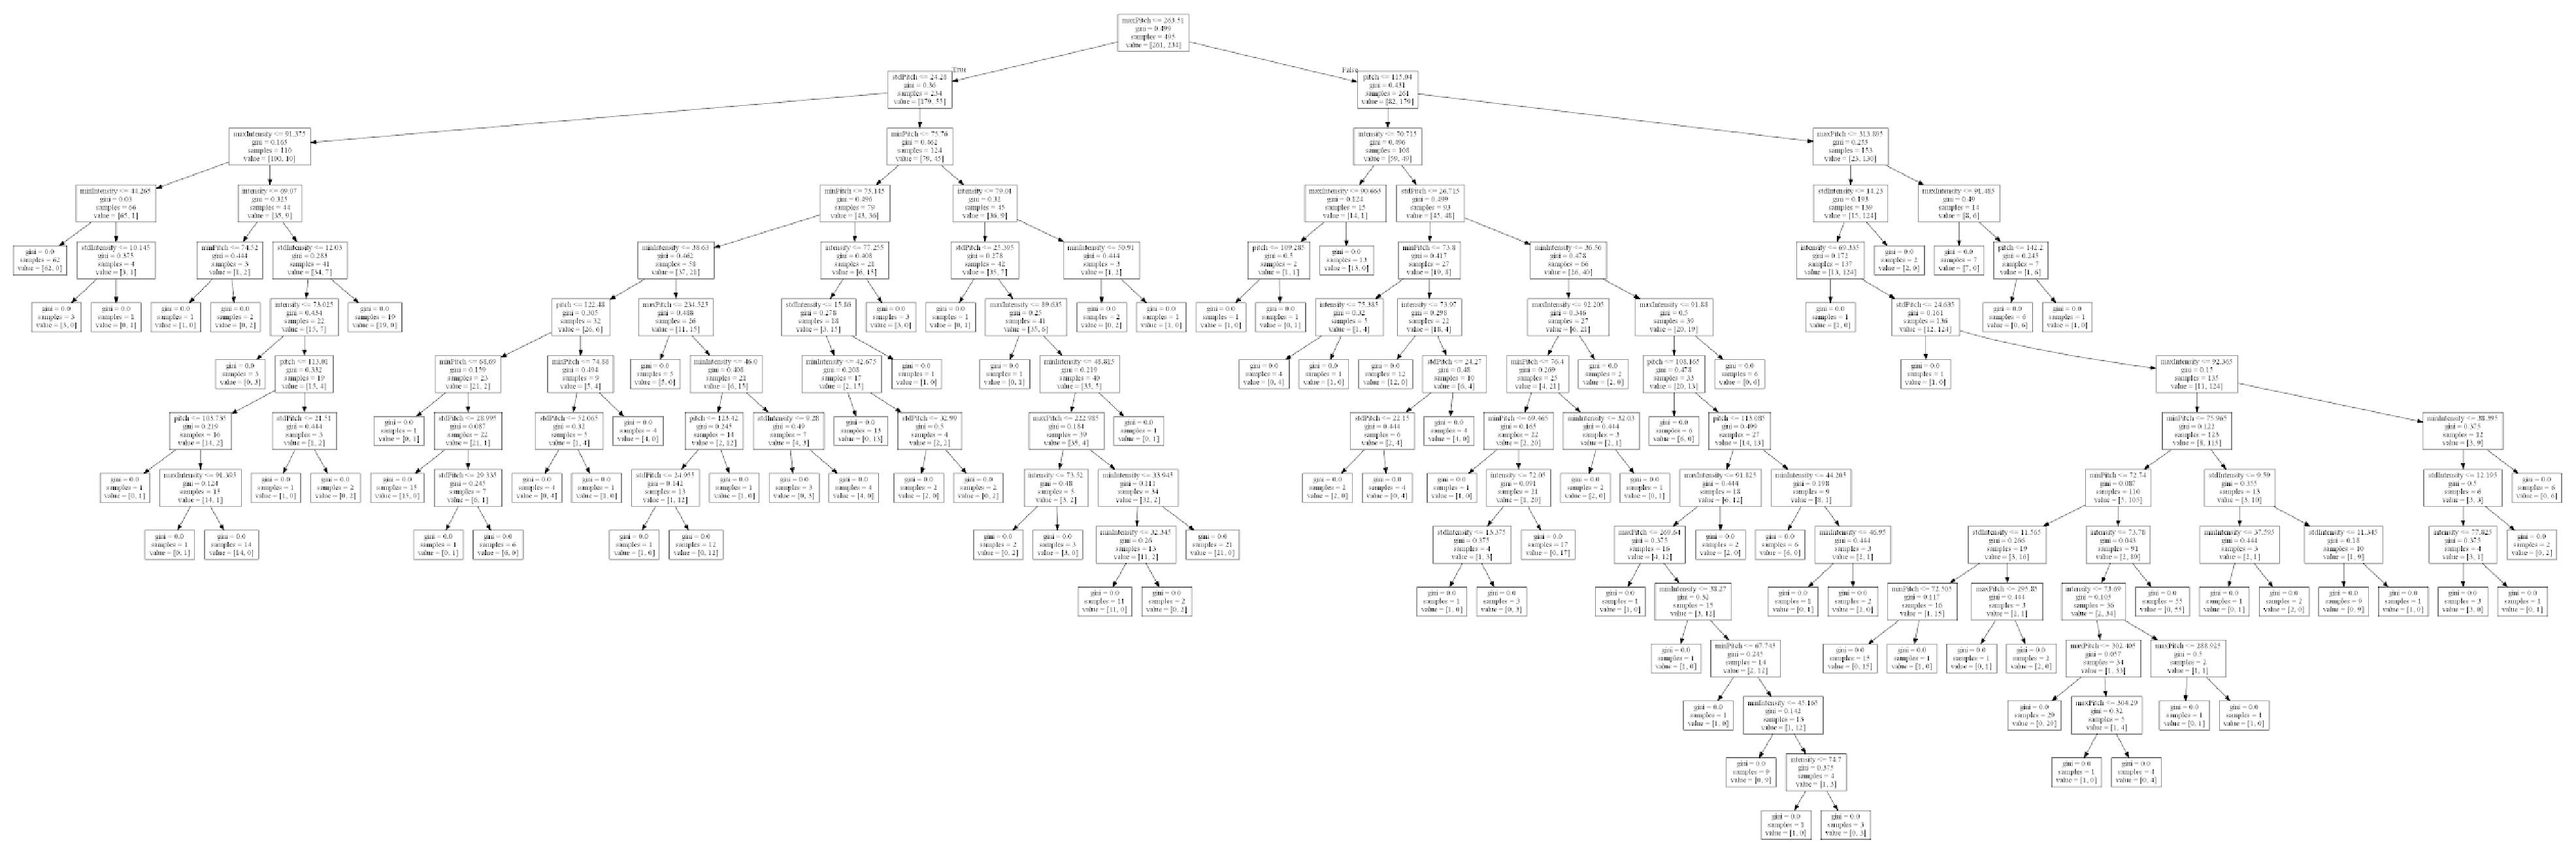
\includegraphics[width=\linewidth]{assets/fig22.eps}
\caption{Mid-Joke Decision Tree}
\end{figure}
\clearpage

\section{Progress Summary}
Our work this term was divided into two distinct parts: analysis of the post-joke audio which expanded on previous work by the robot team and introduction of entirely new functionality for mid-joke audio analysis. We held weekly progress meetings with our client to establish a series of sprints for each branch of the work with defined goals to be achieved by the next meeting.

\subsection{Post-Joke Sprints}

Sprint 1: Jan 8 to Jan 22
\begin{itemize}
\item Split performance recordings into joke and pause audio files
\item Used annotator to classify post-joke data with individual human ratings
\item Created feature extractions from the joke audio files
\item Combined our three human ratings into a ground truth rating for each joke
\end{itemize}

Sprint 2: Jan 22 to Jan 29
\begin{itemize}
\item Combined classification data with feature data
\item Implemented verificaion of joke order per performance in the classifier program
\end{itemize}

Sprint 3: Jan 29 to Feb 12
\begin{itemize}
\item Implemented basic classifiers (SVM, KNN, Decision Tree, Neural Network)
\item Implemented 2-Class and 3-Class
\item Calculated human rater accuracy of individual agreement with the consensus rating
\end{itemize}

Sprint 4: Feb 12 to Feb 26
\begin{itemize}
\item Reannotated all jokes by hand after annotator bug was discovered
\item Implemented normalization in classifier (MinMax, Standardization, Running Average)
\item Performed parameter tuning for SVM classifier
\item Implemented new classifiers (Random Forest, Naive Bayes)
\item Completed CITI training for potential future studies involving human participants (Stretch Goal)
\end{itemize}

Sprint 5: Feb 26 to Mar 11
\begin{itemize}
\item Data visualization
\item Data analysis
\item Working toward moving classifiers onto the robot hardware (Stretch Goal)
\item Preparation for moving framework for the robot from Choregraphe to the Python SDK (Stretch Goal)
\item Began compiling classifier results as foundation for a paper (Stretch Goal)
\end{itemize}

Sprint 6: Mar 11 to Mar 18
\begin{itemize}
\item Completed data visualization
\item Preparation for combining mid-joke and post-joke classifiers
\end{itemize}

\subsection{Mid-Joke Sprints}

Sprint 1: Jan 8 to Jan 22
\begin{itemize}
\item Processed and annotated data from various performances
\item Researched strategies for rating mid-joke laughter
\item Researched how to visualize data
\item Researched various machine learning methods
\item Researched various noise suppression methods; attempted naive method of noise subtraction
\item Learned how to use Jupyter Notebook; used this to start code for unsupervised clustering
\end{itemize}

Sprint 2: Jan 22 to Jan 29
\begin{itemize}
\item Determineed rating system for mid-joke audio (What constitutes a laugh)
\item Decided to use automatic clustering rather than noise suppression
\item Decided on ELAN as the audio annotator tool
\item Extracted audio data from each joke
\item Initially classified extracted data into three groups using K-Means (good, ok, bad)
\item Later shifted to extracting data into two groups (laugh, no laugh)
\end{itemize}

Sprint 3: Jan 29 to Feb 12
\begin{itemize}
\item Annotated jokes for mid-joke laughter
\item Began initial efforts in data clustering (two groups)
\item Analyzed correlation of different audio features
\item Created script to match joke to joke ID
\item Determined which features to extract from mid-joke audio and found their distributions
\end{itemize}

Sprint 4: Feb 12 to Feb 26
\begin{itemize}
\item Looked into Mel-frequency cepstral coefficients (MFCC) to help with better extracting features and detecting laughter
\item Started cross validation algorithm
\item Determined if we needed a baseline approach for mid-joke laughter detection (i.e. look for pitch drop by taking the minimum amplitude and subtracting that from the maximum amplitude)
\item Exported and parsed the annotated data
\item Continued efforts in data clustering
\item Completed CITI training for potential future studies involving human participants (Stretch Goal)
\end{itemize}

Sprint 5: Feb 26 to Mar 11
\begin{itemize}
\item Continued research into MFCC
\item Looked into intensityRange and pitchRange as potential new features to analyze
\item Produced graphs for data visualization
\item Looked into Fourier transformations as possible aid to analysis efforts
\end{itemize}
\clearpage
Sprint 6: Mar 11 to Mar 18
\begin{itemize}
\item Added intensityRange and pitchRange as new features
\item Review jokes that the program classified wrong
\item Categorized errors in the machine learning model into four types: Human annotation error, Post-joke laughter caught in mid-joke audio, Robot laughter caught in audio (only happens with one specific joke), Short laugh heard at beginning of clip
\item Discussed adjusting the timing of the audio segments on the robot or re-annotate the audio to address the errors
\item Produced a visual of data output from simple implementation of MFCC; began interpreting the results
\item Preparation for combining mid-joke and post-joke classifiers
\end{itemize}

\end{document}